\documentclass[tikz,border=2pt]{standalone}
\usepackage{amsmath,amssymb}
\usepackage{pgfplots}
\pgfplotsset{compat=1.18}
\usetikzlibrary{arrows.meta}
\begin{document}
% Exposure offset on log-log axes: E[N_i] = e_i * lambda_i with lambda_i = 0.2 per policy-year, so
% log E[N_i] = log e_i + log 0.2 is a line of slope exactly 1; exposures 10 and 100 give expected counts 2 and 20.
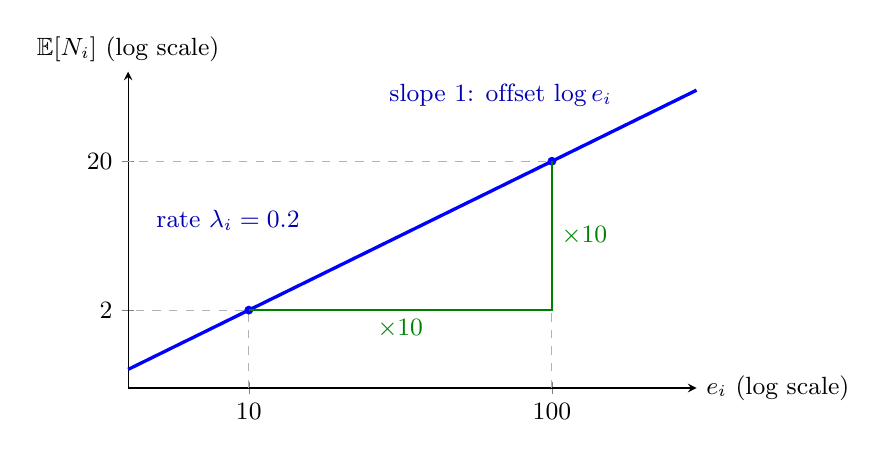
\begin{tikzpicture}[font=\small, >={Latex[length=2mm]}]
  \begin{loglogaxis}[
    axis lines=left, xmin=4, xmax=300, ymin=0.6, ymax=80,
    xtick={10,100}, xticklabels={$10$,$100$},
    ytick={2,20}, yticklabels={$2$,$20$},
    xminorticks=false, yminorticks=false,
    xlabel={$e_i$ (log scale)}, ylabel={$\mathbb E[N_i]$ (log scale)},
    xlabel style={at={(axis description cs:1,0)}, anchor=west},
    ylabel style={rotate=-90, at={(axis description cs:0,1)}, anchor=south},
    width=8.8cm, height=5.6cm, clip=false
    ]
    \addplot[blue, very thick, domain=4:300, samples=2] {0.2*x};
    \draw[gray!60, thin, dashed] (axis cs:10,0.6) -- (axis cs:10,2) -- (axis cs:4,2);
    \draw[gray!60, thin, dashed] (axis cs:100,0.6) -- (axis cs:100,20) -- (axis cs:4,20);
    \fill[blue] (axis cs:10,2) circle (1.6pt);
    \fill[blue] (axis cs:100,20) circle (1.6pt);
    % slope triangle over one factor of 10
    \draw[green!50!black, thick] (axis cs:10,2) -- (axis cs:100,2) -- (axis cs:100,20);
    \node[green!50!black, anchor=north] at (axis cs:31.6,2) {$\times 10$};
    \node[green!50!black, anchor=west] at (axis cs:100,6.3) {$\times 10$};
    \node[blue!70!black, anchor=south east] at (axis cs:170,40) {slope $1$: of\kern0pt fset $\log e_i$};
    \node[blue!70!black, anchor=west] at (axis cs:4.6,8) {rate $\lambda_i=0.2$};
  \end{loglogaxis}
\end{tikzpicture}
\end{document}
